\documentclass[11pt,a4paper,titlepage]{article}
\usepackage[utf8]{inputenc}
\usepackage[margin=2cm,headheight=13.6cm]{geometry}
\usepackage{color}
% Agregados por mi
\usepackage{empheq}
\newcommand*\widefbox[1]{\fbox{\hspace{2em}#1\hspace{2em}}}
\usepackage{ifpdf}
\usepackage{hyperref}
\usepackage{booktabs}
\usepackage{amsmath}
\usepackage{mathtools}
\usepackage{amsfonts}
\usepackage{enumerate}
\usepackage{verbatim}
\usepackage{tikz}
\usetikzlibrary{shapes,snakes}
\newcommand*{\TitleParbox}[1]{\parbox[c]{3.75cm}{#1}}%
\newcommand*{\ntpb}[1]{\parbox[c]{3cm}{#1}}%
\usepackage{multicol}
\usepackage{cancel}
% Command "alignedbox{}{}" for a box within an align environment
% Source: http://www.latex-community.org/forum/viewtopic.php?f=46&t=8144
\newlength\dlf  % Define a new measure, dlf
\newcommand\alignedbox[2]{
% Argument #1 = before & if there were no box (lhs)
% Argument #2 = after & if there were no box (rhs)
&  % Alignment sign of the line
{
\settowidth\dlf{$\displaystyle #1$}  
    % The width of \dlf is the width of the lhs, with a displaystyle font
\addtolength\dlf{\fboxsep+\fboxrule}  
    % Add to it the distance to the box, and the width of the line of the box
\hspace{-\dlf}  
    % Move everything dlf units to the left, so that & #1 #2 is aligned under #1 & #2
\boxed{#1 #2}
    % Put a box around lhs and rhs
}
}

%Para el underbracket con el igual
\newlength\diz  % Define a new measure, diz
\newcommand\alignedunderbracket[2]{
% Argument #1 = before & if there were no box (lhs)
% Argument #2 = after & if there were no box (rhs)
&  % Alignment sign of the line
{
\settowidth\diz{$\displaystyle #1$}  
    % The width of \diz is the width of the lhs, with a displaystyle font
\addtolength\diz{\fboxsep+\fboxrule}  
    % Add to it the distance to the box, and the width of the line of the box
\hspace{-\diz}  
    % Move everything diz units to the left, so that & #1 #2 is aligned under #1 & #2
\underbracket{#1 #2}
    % Put a box around lhs and rhs
}
}

%Fin de agregados por mi
\usepackage{listings}
\usepackage{graphicx}
\usepackage[spanish]{babel}
\usepackage{caption}
\usepackage{subcaption}
\usepackage{float}
\usepackage{titling}
\usepackage{pgfkeys}
\definecolor{mygreen}{RGB}{0,127,0}
\definecolor{mygray}{RGB}{100,100,100}
\definecolor{mymauve}{RGB}{100,32,255}
\definecolor{lgray}{RGB}{230,230,230}
\lstset{ %
  frame=none,
  backgroundcolor=\color{white},   % choose the background color; you must add \usepackage{color} or \usepackage{xcolor}
  basicstyle=\footnotesize\ttfamily,        % the size of the fonts that are used for the code
  breakatwhitespace=false,         % sets if automatic breaks should only happen at whitespace
  breaklines=true,                 % sets automatic line breaking
  captionpos=t,                    % sets the caption-position to bottom
  commentstyle=\color{mygreen},    % comment style
  deletekeywords={...},            % if you want to delete keywords from the given language
  escapeinside={\%*}{*)},          % if you want to add LaTeX within your code
  extendedchars=true,              % lets you use non-ASCII characters; for 8-bits encodings only, does not work with UTF-8
%  frame=single,                    % adds a frame around the code
  keepspaces=true,                 % keeps spaces in text, useful for keeping indentation of code (possibly needs columns=flexible)
  keywordstyle=\color{blue},       % keyword style
  language=,                 % the language of the code
  morekeywords={*,...},            % if you want to add more keywords to the set
  numbers=left,                    % where to put the line-numbers; possible values are (none, left, right)
  numbersep=5pt,                   % how far the line-numbers are from the code
  numberstyle=\tiny\color{mygray}, % the style that is used for the line-numbers
  rulecolor=\color{black},         % if not set, the frame-color may be changed on line-breaks within not-black text (e.g. comments (green here))
  showspaces=false,                % show spaces everywhere adding particular underscores; it overrides 'showstringspaces'
  showstringspaces=false,          % underline spaces within strings only
  showtabs=false,                  % show tabs within strings adding particular underscores
  stepnumber=1,                    % the step between two line-numbers. If it's 1, each line will be numbered
  stringstyle=\color{mymauve},     % string literal style
  tabsize=4,                       % sets default tabsize to 2 spaces
  aboveskip=3mm,
  belowskip=3mm,
}

\usepackage{fancyhdr}
\pagestyle{fancy}
\rhead{}
\usepackage{datetime}
\usepackage{moresize}

\newdateformat{monthyeardate}{%
  \monthname[\THEMONTH] \THEYEAR}

\newcommand{\rulebreak}{%
	\par%
	\vspace{0.9cm}%
    \noindent\rule{4cm}{0.4pt}%
    \vspace{1.2cm}%
    \par%
}

\newcommand{\coverpage}[1]{%
	\pagenumbering{roman}%
	\thispagestyle{empty}%
	\lhead{\textsc{\small{TP 1:} #1}}%
    \title{Diseño Analógico de Circuitos Integrados}%
    \author{Autor: Leandro Marsó,
    \\
            Profesores: Benjamín Reyes}%
    \newgeometry{left=5cm,bottom=2cm,right=5cm,top=2cm}%
	\begin{center}\hspace{0pt}\vfill%
    \uppercase{
    Universidad Nacional de Córdoba\\
    Facultad de Ciencias Exactas, Físicas y Naturales
    }
	\rulebreak%
    {\Large\textbf{Diseño Analógico de Circuitos Integrados}}
    
    \vspace{0.5cm}
    {\HUGE\textbf{\textit{#1}}}
    
    \vspace{0.5cm}
	\theauthor%
	\par%
	\vspace{0.9cm}%
    \noindent\rule{4cm}{0.4pt}%
    \vspace{0.45cm}
    \tableofcontents%
	\rulebreak%
    \monthyeardate\today\par
    \hspace{0pt}
	\end{center}%
    \vfill
    \hspace{0pt}
	\pagebreak%
    \restoregeometry%
    \pagenumbering{arabic}%
}

% Custom arguments for /fig command
\pgfkeys{
 /fig/.is family, /fig,
 default/.style = 
  {scale = 1,
   angle = 0},
 scale/.estore in = \figScale,
 angle/.estore in = \figAngle
}
\newcommand{\fig}[2][]{%
	\pgfkeys{/fig, default, #1}%
	\begin{figure}[H]%
    \centering
    \includegraphics[angle=\figAngle,width=\figScale\textwidth]{#2}%
	\end{figure}%
}

\newcommand{\filename}[1]{%
	\texttt{#1}%
}

\newcommand{\vhdl}[1]{%
  \lstinputlisting[language=vhdl]{#1}
}

\newcommand*\paths[1]{\lstset{inputpath=#1}\graphicspath{#1}}


\everymath{\displaystyle} %Esto es para que la matemática dentro de texto sea más grande que el texto

\begin{document}
\coverpage{TP 1}
  
\subsection{Canal Corto vs. Canal largo}
Comparación de curvas del NMOS para canal largo y canal corto.
%Comparar las curvas del NMOS (Ver circuito Fig. 2) para canal largo (L=3um y L=6um)
%y canal corto (L=0.6um). Calcular el W según corresponda.
%• NMOS canal corto: L=0.6um y relación W/L=5.
%• NMOS canal largo: L=3um y relación W/L=5.
%• NMOS canal largo: L=6um y relación W/L=5.
%Obtener las siguientes curvas para una comparativa canal corto/largo:
%• I D vs. V GS (escala lineal).
%• I D (escala Log) vs. V GS .
%• I D vs. V DS , barriendo V GS de forma paramétrica.
%• gm/ I D vs. I D
%• gm/ I D vs. I D (escala Log)

%Las tareas se crean en el main y se definen por fuera. La tarea \verb|vLEDTask1| enciende/apaga un led con un período de \verb|configTICK_RATE_HZ / 6|.

%La tarea \verb|vLEDTask2| enciende/apaga otro led en un período de \verb|configTICK_RATE_HZ / 14|.
%
%La tarea \verb|vUARTTask| imprime por la salida estandar de debugueo el texto \verb|Tick: contador|, siendo \verb|contador| un entero que se incrementa cada \verb|configTICK_RATE_HZ|.
 
%Las tres tareas tienen la misma prioridad: \verb|tskIDLE_PRIORITY| que está definido en el archivo \verb|task.h| con un valor de cero.
 
%\verb|configTICK_RATE_HZ| está definido en el archivo \verb|FREERTOSConfig.h| con el valor de 1000. Estando el tick definido en un milisegundo. 

\vspace{0.3cm}
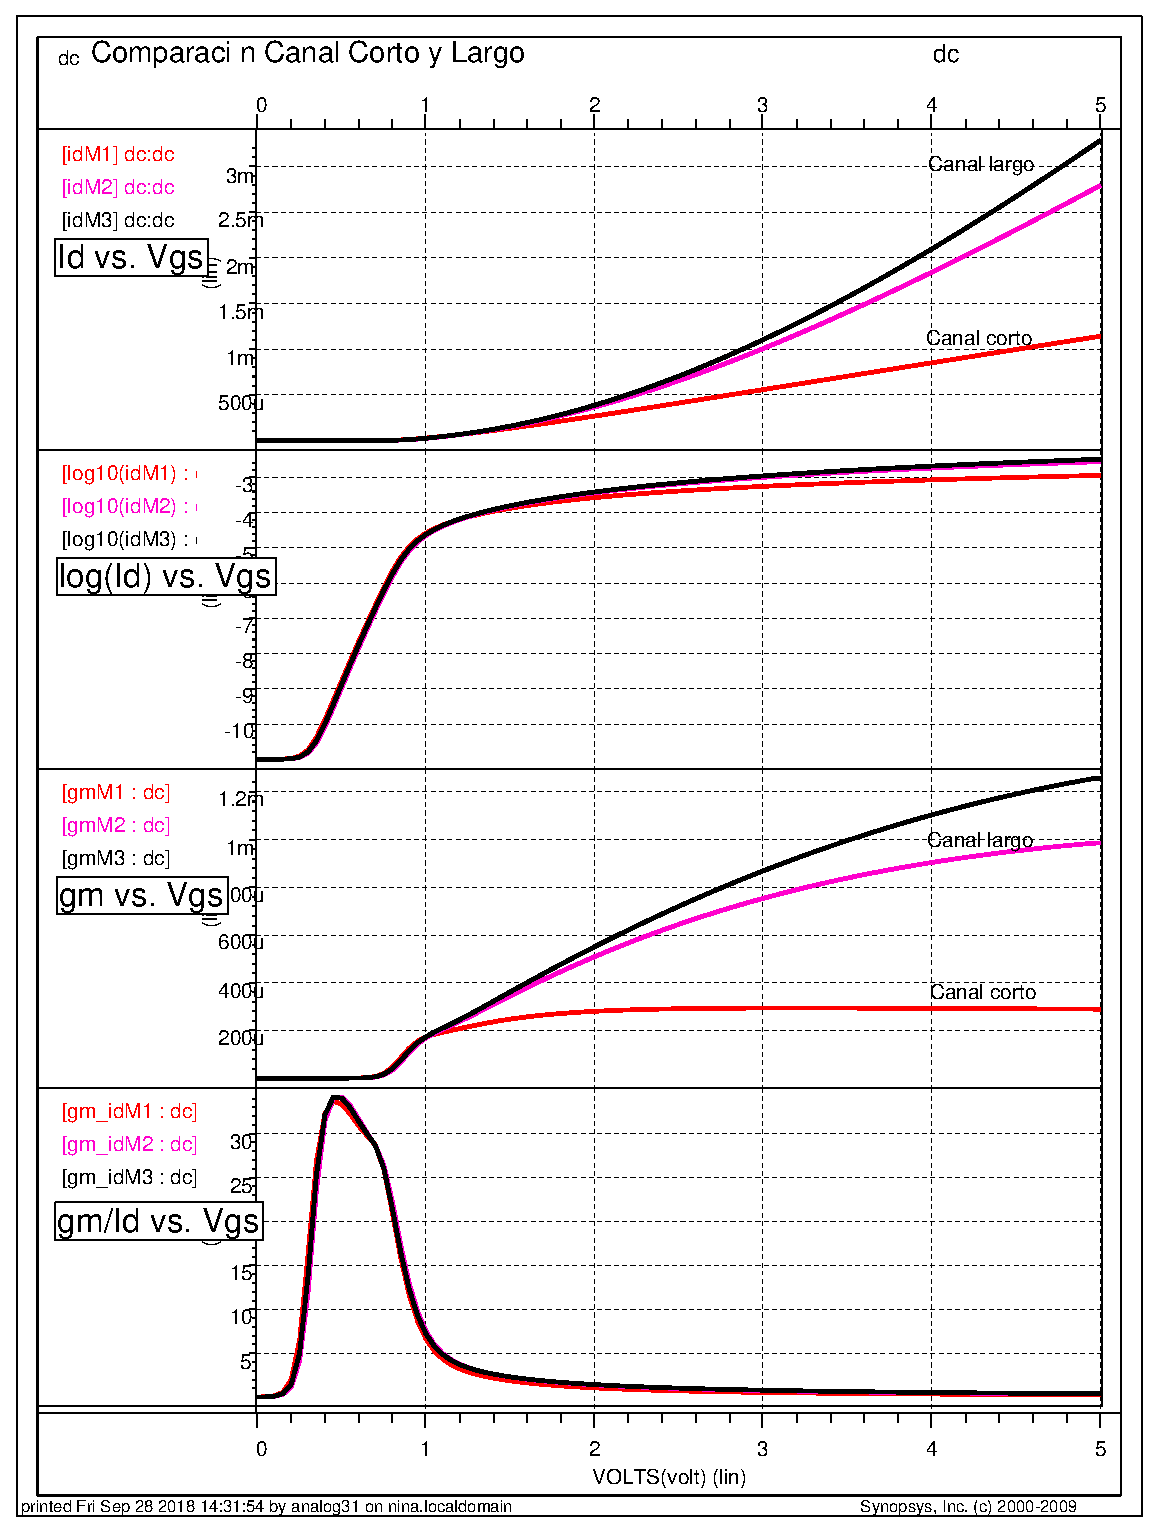
\includegraphics[scale=0.4, angle=0]{images/todas}
\captionof{figure}{$I_D$ vs. $V_{GS}$ (escala lineal)}
\vspace{0.3cm}
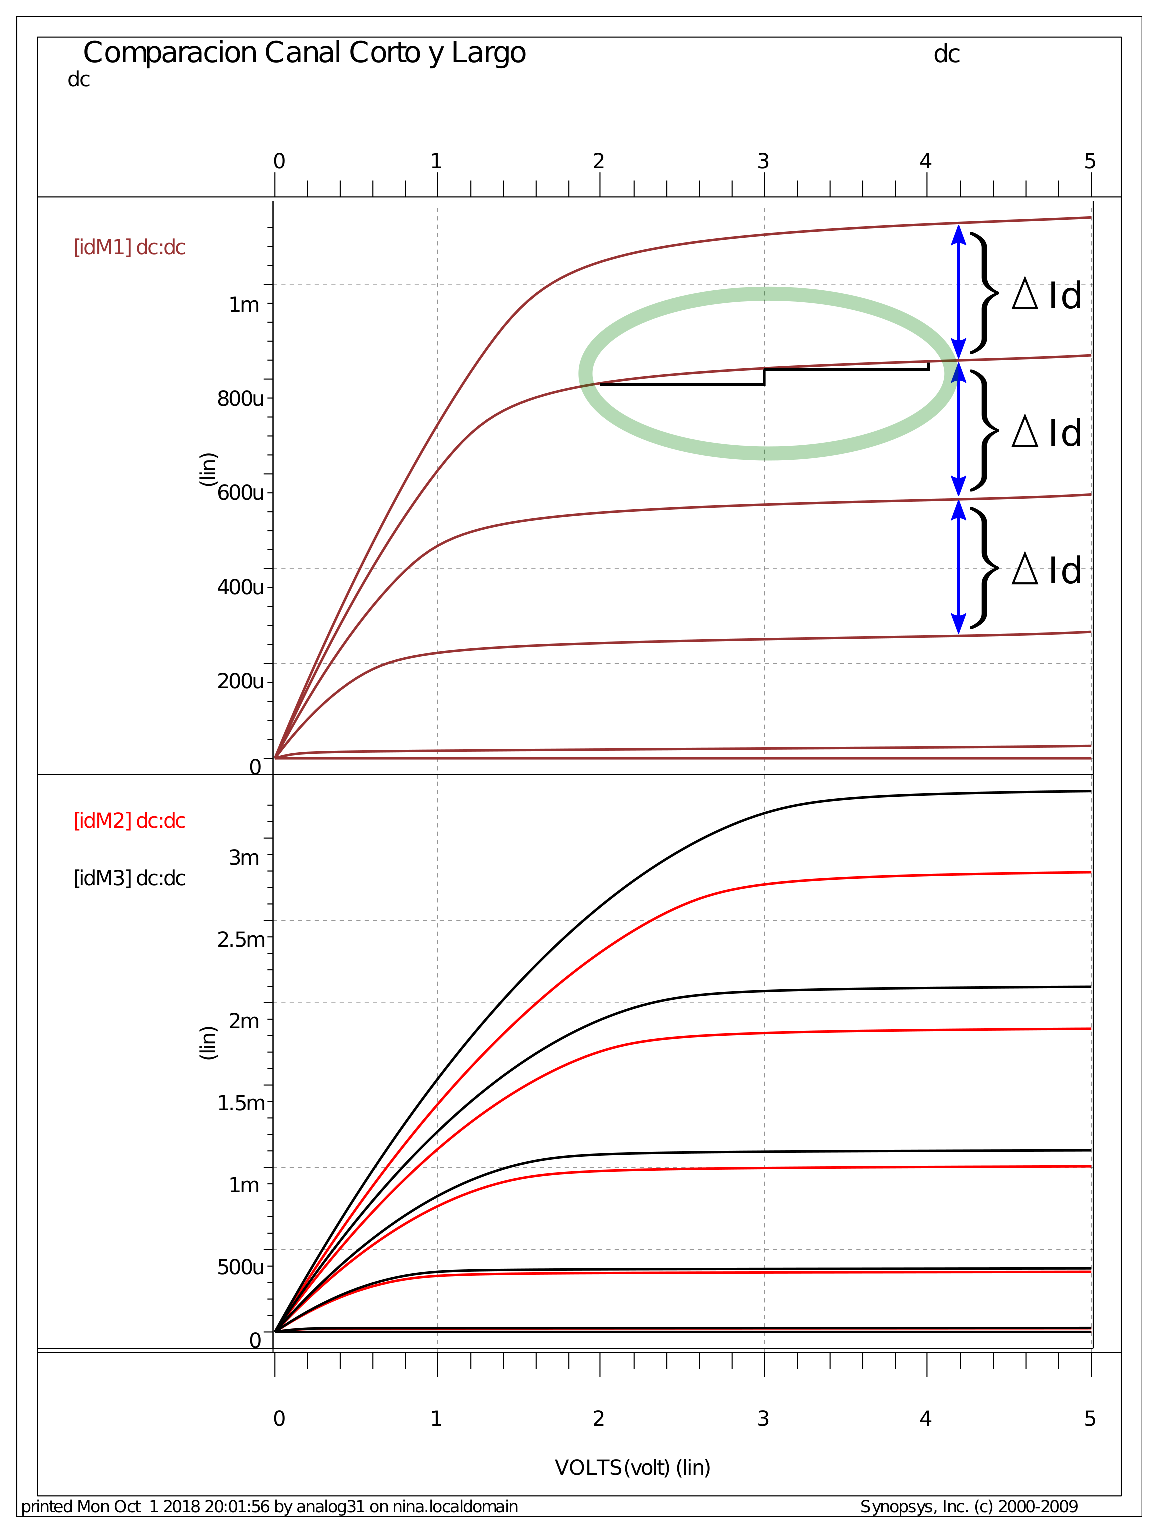
\includegraphics[scale=0.4, angle=-90]{images/parametric}
\captionof{figure}{$I_D$ vs. $V_{DS}$ , barriendo $V_{GS}$ de forma paramétrica}
\subsubsection{$I_D$ vs. $V_{GS}$} 
\begin{itemize}
	\item $V_{th}$ de M1 ($L=0.6\mu$m): $0.674243$V
	\item $V_{th}$ de M2 ($L=3\mu$m): $0.69121$V
	\item $V_{th}$ de M3 ($L=6\mu$m): $0.680835$V
\end{itemize}



%%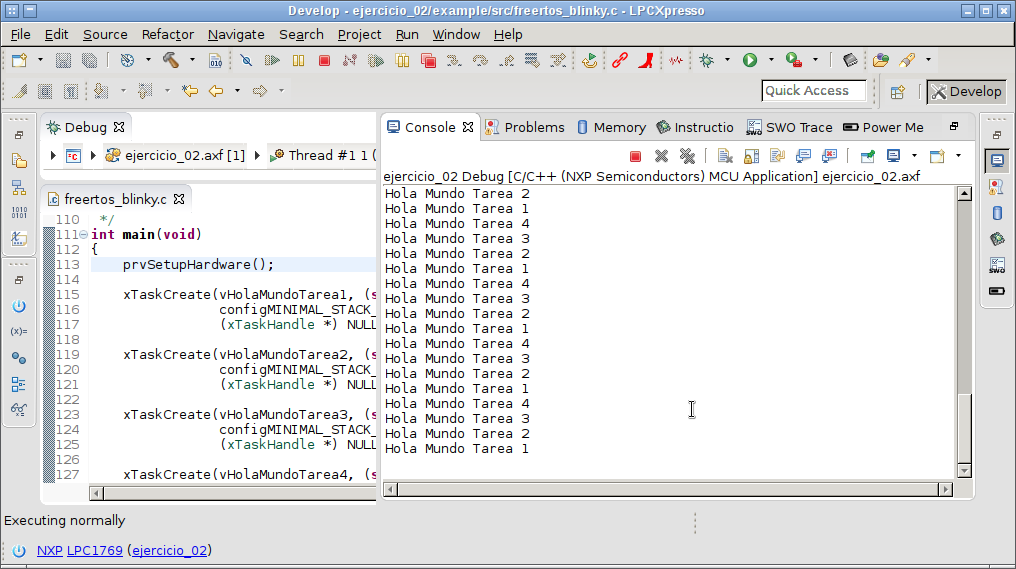
\includegraphics[scale=0.7, angle=90]{images/tp_3_2}
%%\captionof{figure}{bla}

%\vspace{1cm}

%\subsubsection*{Ejercicio 2}
%Cuando todas las tareas tienen igual prioridad, el orden es: Tarea 4, 1, 2 y 3. Al poner prioridad máxima a la 4 y mínima a la tarea 1, Se ejecutó tarea 4, 3, 2 y 1. Al cambiar la prioridad a todas las tareas, sucedió que el orden en que se ejecutaron las tareas sigue la definición de prioridades. 
%
%\vspace{0.2cm}
%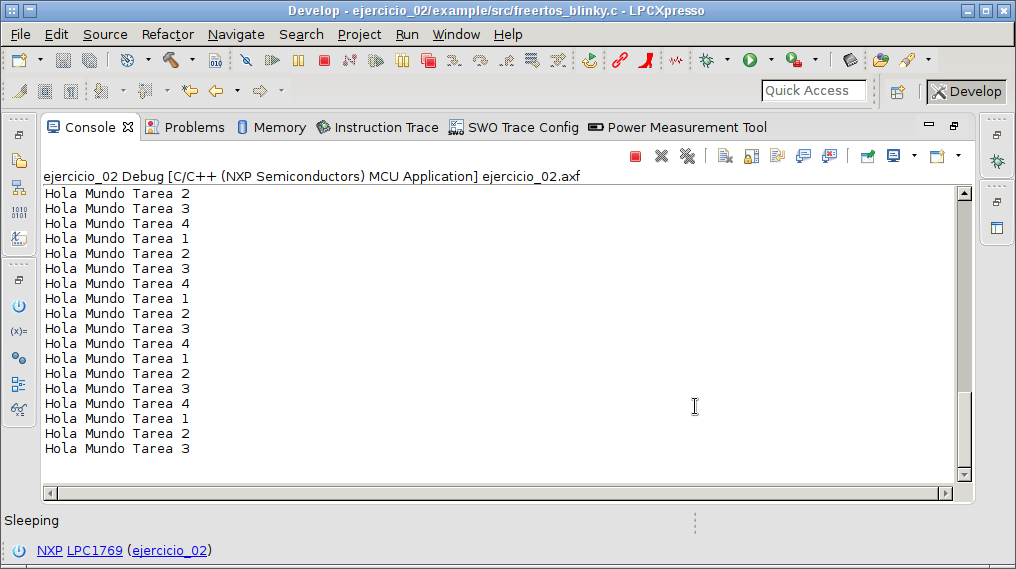
\includegraphics[scale=0.34]{images/tp_3}
%\captionof{figure}{Captura de pantalla con secuencia 4, 1, 2, 3, ...}
%\vspace{0.2cm}
%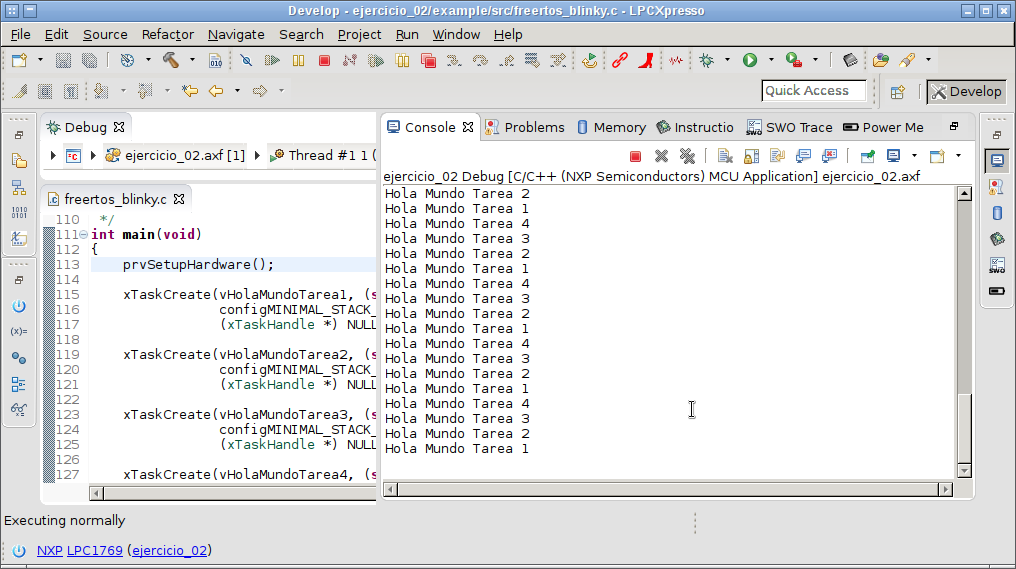
\includegraphics[scale=0.4]{images/tp_3_2}
%\captionof{figure}{Captura de pantalla luego de reasignación de prioridades.}
%\vspace{0.5cm}

%\subsubsection*{Ejercicio 3}
%Agregamos una tarea más, y también creamos una variable global para guardar el \emph{handle} de la tarea 1 (ver línea 8), para poder suspenderla y reanudarla desde la tarea 5 (ver línea 82 y 87):
%\lstinputlisting[language=C, firstline=32]{src/ejercicio_3.c}
%% Otro parámetro, por si es necesario cortar el archivo: lastline=157 
%
%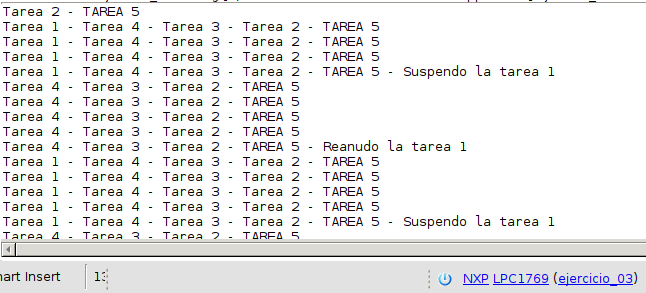
\includegraphics[scale=0.4]{images/tp_3_ej3}
%\captionof{figure}{Usando la impresión por pantalla para ver el efecto de suspender/reanudar una tarea...}
%\vspace{0.2cm}
%
%\paragraph{Comentarios}
%Las tareas se ejecutan según las prioridades asignadas, y es posible verlo a simple vista cuando utilizamos la salida por terminal con la función \verb|DEBUGOUT|. Pero cuando las tareas sólo encienden/apagan los leds, el resultado es un parpadeo conjunto de todos los leds. No se perciben el orden en que se realizan las tareas. Tal funcionamiento es el esperado, y podemos decir que a simple vista las 5 tareas se realizan al mismo tiempo.
%
%\subsubsection*{Ejercicio 4}
%En la \emph{tarea 5} agregamos el siguiente código:
%\lstinputlisting[language=C, firstline=118, lastline=122]{src/ejercicio_4.c}
%La salida por terminal es la siguiente:
%
%\includegraphics[scale=0.4]{images/tp_3_ej4}
%%\captionof{figure}{Usando la impresión por pantalla para ver el efecto de suspender/reanudar una tarea...}
%\vspace{0.2cm}
%\paragraph{Comentarios:}
%Eliminar una tarea es muy fácil. Dos cosas a tener en cuenta: 
%\begin{itemize}
%    \item Intentar eliminar dos veces una tarea genera un \emph{hard Fault}.
%    \item La memoria que se reserva con \emph{malloc} debe liberarse antes de eliminar la tarea. Y para liberar la zona de memoria utilizada por el \emph{kernel} para la tarea, debe estar habilitada la tarea \emph{idle}.
%\end{itemize}
%\subsubsection*{Ejercicio 5}
%En este ejercicio, nuestro objetivo fué crear una cola de 5 items, para guardar un mensaje de hasta 40 caracteres. Esto lo hicimos en la línea 113. Luego, 3 tareas insertan un mensaje en la cola, como se puede ver en las líneas 37, 53 y 69. En otra tarea, vaciamos la cola imprimiendo cada mensaje, como se puede ver en las líneas 89 hasta 99.
%\lstinputlisting[language=C, firstline=31 ]{src/ejercicio_05.c}
%\subsubsection*{Ejercicio 6}
%En este ejercicio, creamos un semáforo en la línea 41. Mientras el pulsador no se acciona, este semáforo no puede ser tomado (línea 45), ya que en la ISR se ejecuta el \emph{give} (línea 22).
%\lstinputlisting[language=C]{src/ejercicio_06.c}
\end{document}
